\documentclass[10pt]{beamer}
% \usetheme{Boadilla}
  \usetheme{default}


% acronyms for text or math mode
\newcommand {\ccast} {\mbox{\small CCAST}}
\newcommand {\cris} {\mbox{\small CrIS}}

\newcommand {\airs} {\mbox{\small AIRS}}
\newcommand {\iasi} {\mbox{\small IASI}}
\newcommand {\idps} {\mbox{\small IDPS}}
\newcommand {\nasa} {\mbox{\small NASA}}
\newcommand {\noaa} {\mbox{\small NOAA}}
\newcommand {\nstar} {\mbox{\small STAR}}
\newcommand {\umbc} {\mbox{\small UMBC}}
\newcommand {\uw}   {\mbox{\small UW}}

\newcommand {\fft}  {\mbox{\small FFT}}
\newcommand {\ifft} {\mbox{\small IFFT}}
\newcommand {\fir}  {\mbox{\small FIR}}
\newcommand {\fov}  {\mbox{\small FOV}}
\newcommand {\for}  {\mbox{\small FOR}}
\newcommand {\ict}  {\mbox{\small ICT}}
\newcommand {\ils}  {\mbox{\small ILS}}
\newcommand {\igm}  {\mbox{\small IGM}}
\newcommand {\opd}  {\mbox{\small OPD}}
\newcommand {\rms}  {\mbox{\small RMS}}
\newcommand {\zpd}  {\mbox{\small ZPD}}
\newcommand {\ppm}  {\mbox{\small PPM}}
\newcommand {\srf}  {\mbox{\small SRF}}
\newcommand {\sdr}  {\mbox{\small SDR}}

\newcommand {\ES} {\mbox{\small ES}}
\newcommand {\SP} {\mbox{\small SP}}
\newcommand {\IT} {\mbox{\small IT}}
\newcommand {\SA} {\mbox{\small SA}}

\newcommand {\ET} {\mbox{\small ET}}
\newcommand {\FT} {\mbox{\small FT}}

\newcommand {\wn} {\mbox{cm$^{-1}$}}

% abbreviations, mainly for math mode
\newcommand {\real} {\mbox{real}}
\newcommand {\imag} {\mbox{imag}}
\newcommand {\atan} {\mbox{atan}}
\newcommand {\obs}  {\mbox{obs}}
\newcommand {\calc} {\mbox{calc}}
\newcommand {\sinc} {\mbox{sinc}}
\newcommand {\psinc} {\mbox{psinc}}
\newcommand {\std} {\mbox{std}}

% symbols, for math mode only
\newcommand {\lmax} {L_{\mbox{\tiny max}}}
\newcommand {\vmax} {V_{\mbox{\tiny max}}}

\newcommand {\tauobs} {\tau_{\mbox{\tiny obs}}}
\newcommand {\taucal} {\tau_{\mbox{\tiny calc}}}
\newcommand {\Vdc}  {V_{\mbox{\tiny DC}}}

\newcommand {\rIT} {r_{\mbox{\tiny\textsc{ict}}}}
\newcommand {\rES} {r_{\mbox{\tiny\textsc{es}}}}
\newcommand {\robs} {r_{\mbox{\tiny obs}}}

\newcommand {\rITobs} {r_{\mbox{\tiny\textsc{ict}}}^{\mbox{\tiny obs}}}
\newcommand {\rITcal} {r_{\mbox{\tiny\textsc{ict}}}^{\mbox{\tiny cal}}}

\newcommand {\ITmean} {\langle\mbox{\small IT}\rangle}
\newcommand {\SPmean} {\langle\mbox{\small SP}\rangle}


\title{AIRS deconvolution and the \\
       translation of AIRS to CrIS radiances \\ 
}
\author{H.~E.~Motteler, L.~L.~Strow}
\institute{
  UMBC Atmospheric Spectroscopy Lab \\
  Joint Center for Earth Systems Technology \\
}
\date{\today}
\begin{document}

%----------- slide --------------------------------------------------%
\begin{frame}[plain]
\titlepage
\end{frame}
%----------- slide --------------------------------------------------%
\begin{frame}
\frametitle{introduction}
\begin{itemize}

  \item Upwelling infrared radiation as measured by {\airs},
    {\cris}, and {\iasi} is a significant part of the long term
    climate record.

  \item These instruments have broadly similar spatial sampling and
    spectral resolution, channel response functions, and band spans.

  \item We make regular use of {\airs} to {\cris} and {\iasi} to
    {\cris} translations, and have implemented and tested {\iasi} to
    {\airs} and {\cris} to {\airs} translations as well.  But aside
    from {\airs} to {\cris} the methods used are for the most part
    conventional.

  \item {\airs} is a grating spectrometer with a distinct response
    function for each channel, while {\cris} is a Michaelson
    interferometer with a sinc response function after calibration
    and corrections.

  \item We use our detailed knowledge of the {\airs} spectral
    response functions to deconvolve {\airs} channel radiances to a
    resolution enhanced intermediate representation.

  \item This intermediate representation is then reconvolved to
    {\cris} or other instrument specifications.

\end{itemize}
\end{frame}
%----------- slide --------------------------------------------------%
\begin{frame}
\frametitle{AIRS spectral response functions}
\begin{itemize}

  \item Each {\airs} channel $i$ has an associated spectral response
    function or {\srf} $\sigma_i(v)$, a function of frequency $v$.

  \item Channel radiance $c_i = \int \sigma_i(v)r(v)\,dv$, where $r$
    is radiance at frequency $v$.

  \item The center or peak of $\sigma_i$ is the nominal channel
    frequency.

  \item We can approximate the {\airs} {\srf}s with a generalized
    Gaussian of the form \[w(v, v_0, \fwhm) =
    \exp\left(-\left(\frac{(v - v_0)^2}{2c^2}\right)^{1.5}\right) \]
    where $c=\fwhm / (2\sqrt{2\ln 2})$ and $v_0$ is the desired
    channel center.

  \item The exponent $1.5$ was chosen to give an approximate match
    to {\airs} {\srf}s with the same {\FWHM} and channel centers,
    though without the fine structure and variation.

\end{itemize}
\end{frame}
%----------- slide --------------------------------------------------%
\begin{frame}
\frametitle{sample SRFs and resolving power}
\begin{columns}[t]
\begin{column}{0.5\textwidth}
  \begin{centering}
  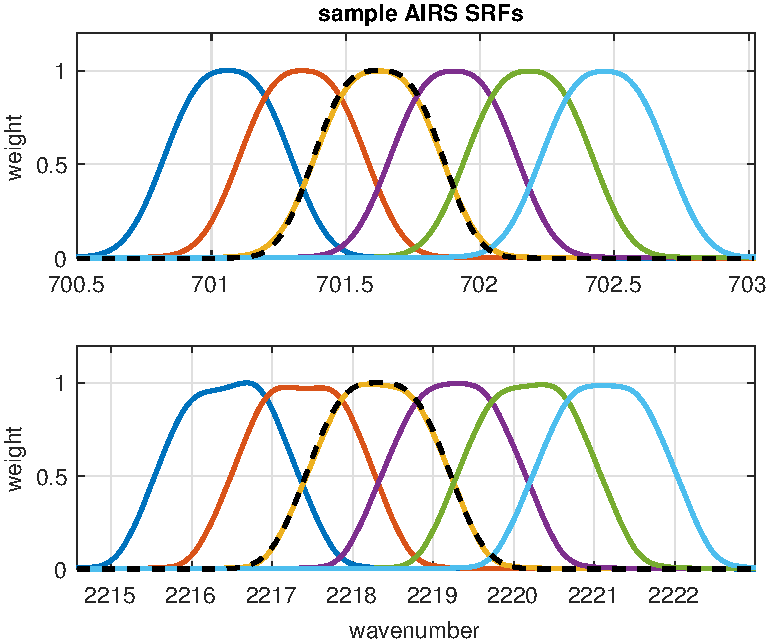
\includegraphics[width=\textwidth]{figures/airs_sample_SRF.pdf} \\
  \end{centering}\vspace{2mm}
  Sample {\airs} spectral response functions from the low and high
  ends of the band.  The dashed line is the generalized Gaussian
  function.

\end{column}
\begin{column}{0.5\textwidth}  
  \begin{centering}
  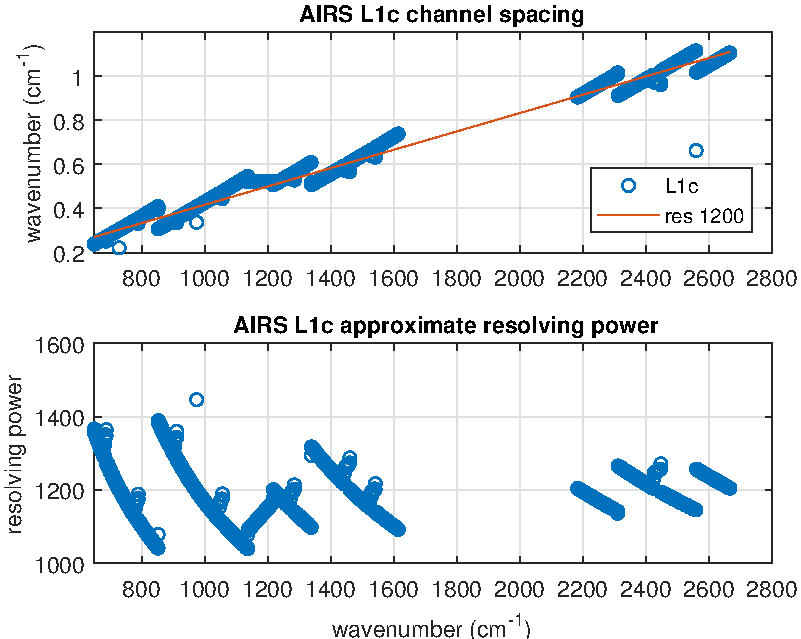
\includegraphics[width=\textwidth]{figures/airs_L1c_res.pdf}
  \end{centering}\vspace{3mm}
  {\airs} L1c channel spacing and resolving power, $R =
  v_i/\fwhm_i$.  The relatively regular L1c channel spacing aids the
  deconvolution. 

\end{column}
\end{columns}
\end{frame}
%----------- slide --------------------------------------------------%
\begin{frame}
\frametitle{the AIRS deconvolution}
\begin{itemize}

  \item Let $\vec v_b = v_1,v_2,\ldots,v_m$ be a $0.1~\wn$ grid
    spanning the domains of the functions $\sigma_i$.

  \item This is the approximate resolution of the {\srf}
    measurements and is convenient for reconvolution to the {\cris}
    user grid.

  \item Let $S_b$ be an $n\times m$ array where row $i$ is
    $\sigma_i(v)$ tabulated at the $\vec v_b$ grid, with rows
    normalized to~1.

  \item Note that the $\sigma_i(v)$ here are the measured {\srf}s,
    not our Gaussian approximation.

  \item If $r$ is radiance at the $\vec v_b$ grid, then $c = S_b r$
    is a reasonable approximation of $\int\sigma_i(v)r(v)\,dv$.

  \item We want to start with $c$ and find $r$, that is to
    deconvolve $c$ by solving $S_b r = c$ for $r$.  

  \item Since $n < m$ the system is underdetermined.  

\end{itemize}
\end{frame}
%----------- slide --------------------------------------------------%
\begin{frame}
\frametitle{the AIRS deconvolution}
\begin{itemize}

  \item We take the Moore-Penrose pseudoinverse of $S_b$ to get $r_0
    = S_b^{-1} c$.

  \item This gives a minimal solution, in the sense that $||r_0||_2
     \le ||r_j||_2$ for all $r_j$ satisfying $S_b r_j = c$.  

  \item The condition number for $S_b$ as built from the L1c
    channels is $||S_b||_2||S_b^{-1}||_2 = 115$, which is tolerable.

  \item Although our main goal is to reconvolve the $0.1~\wn$
    intermediate representation to the {\cris} or other user grids,
    we first compare the deconvolved radiances with reference truth
    from a direct convolution to the intermediate grid.

  \item We use the generalized Gaussian as reference truth for the
    $0.1~\wn$ intermediate grid with ${\fwhm} = v_i / 2000$, where
    $v_i$ are the grid frequencies.  

  \item This represents a hypothetical grating spectrometer with a
    resolving power of 2000, oversampled to the 0.1~\wn\ grid.

\end{itemize}
\end{frame}
%----------- slide --------------------------------------------------%
\begin{frame}
\frametitle{examples of deconvolution}
\begin{columns}[t]
\begin{column}{0.5\textwidth}
  \begin{centering}
  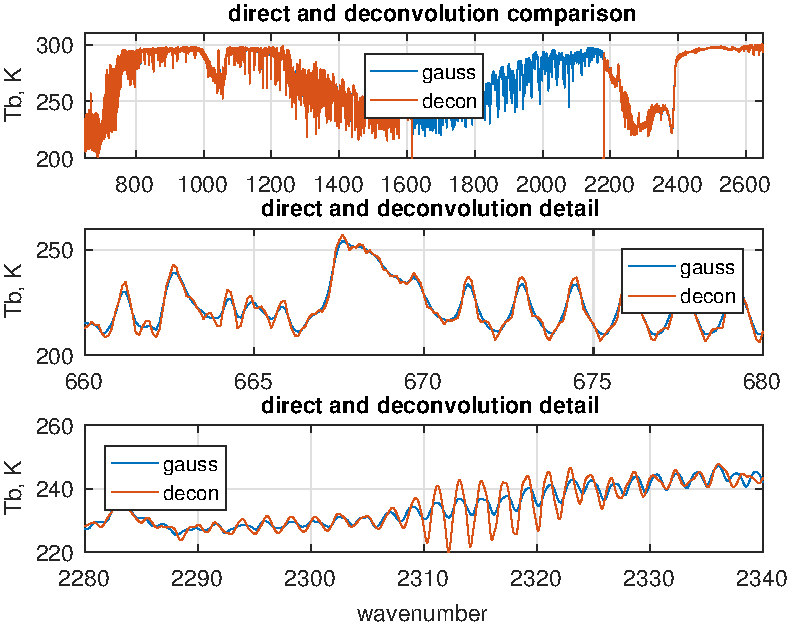
\includegraphics[width=\textwidth]{figures/airs_decon_spec.pdf}
  \end{centering}\vspace{3mm}
  Spectra from fitting profile 1 for direct convolution to the
  $0.1$~\wn\ grid and for deconvolved {\airs}.  We see some
  overshoot and ringing in the deconvolution.

\end{column}
\begin{column}{0.5\textwidth}  
  \begin{centering}
  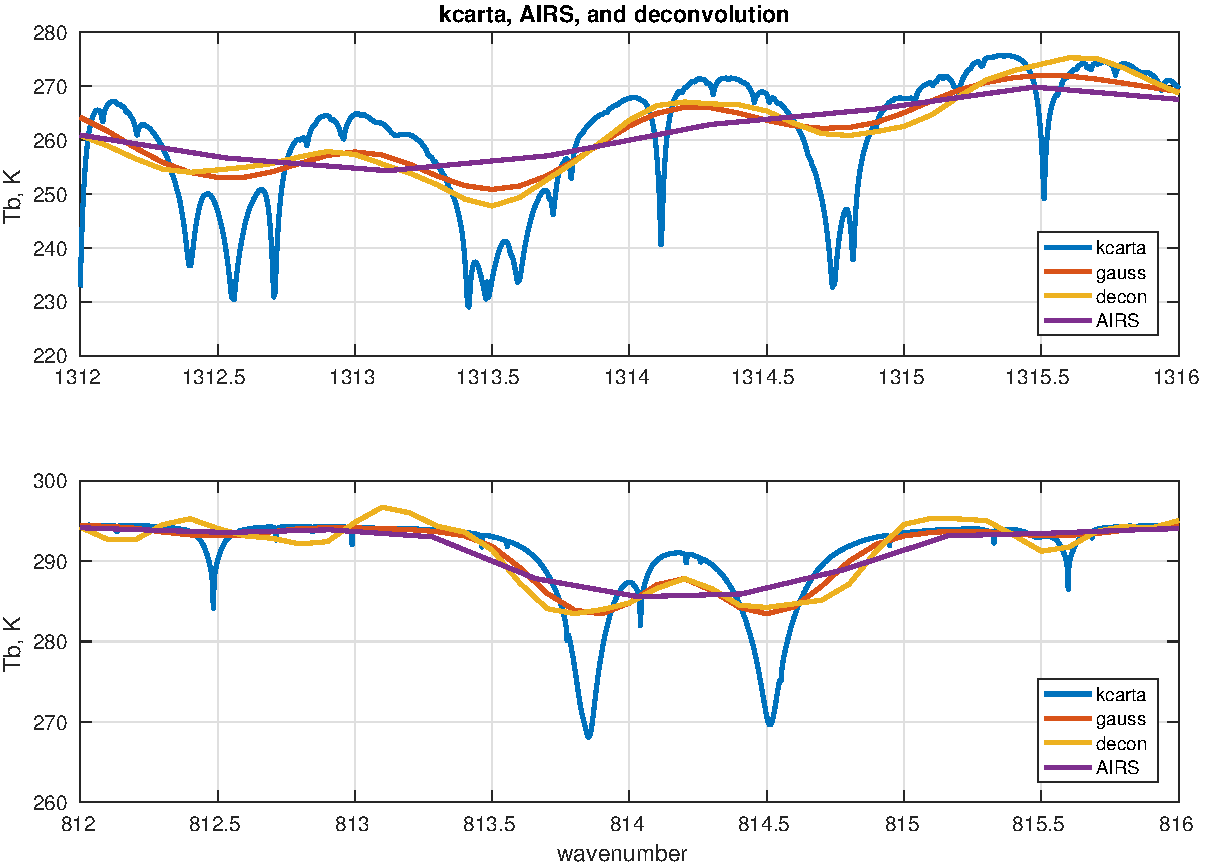
\includegraphics[width=\textwidth]{figures/airs_decon_zoom.pdf}
  \end{centering}\vspace{2mm}
  Details from fitting profile 1 for kcarta, direct convolution to
  the $0.1$~\wn\ grid, deconvolved {\airs}, and true {\airs}.  The
  deconvolution restores some detail.
\end{column}
\end{columns}
\end{frame}
%----------- slide --------------------------------------------------%
\begin{frame}
\frametitle{deconvolution notes}
\begin{itemize}

  \item The {\airs} deconvolution gives a modest resolution
    enhancement, at the cost of added artifacts and noise.

  \item The deconvolution captures some fine structure that is
    present in the direct convolution but not the AIRS L1c spectra,
    and can resolves lines that are merged in the {\airs} data.

  \item But we also see some ringing and overshoot that is not
    present in the direct convolution.

  \item These artifacts are acceptable because we do not propose
    using the deconvolved radiances directly; they are an
    intermediate step before reconvolution to a lower resolution.

\end{itemize}
\end{frame}
%----------- slide --------------------------------------------------%
\begin{frame}
\frametitle{AIRS to CrIS translation}
\begin{itemize}

  \item Given {\airs} deconvolution to a $0.1~\wn$ intermediate
    grid, reconvolution to the {\cris} user grid is straightforward.

  \item For the {\cris} standard resolution the channel spacing is
    $0.625~\wn$ for the LW band, $1.25~\wn$ for the MW, and
    $2.5~\wn$ for the SW.

  \item For each {\cris} band, we 
    \begin{enumerate}
       \item find the {\airs} and {\cris} band intersection, 
       \item apply a bandpass filter to the deconvolved {\airs}
         radiances restricting them to the intersection, with a
         rolloff outside the intersection, and
       \item reconvolve the filtered spectra to the {\cris} user
         grid with a zero-filled double Fourier transform
    \end{enumerate}

  \item The translation above is from {\airs} to unapodized {\cris},
    but we will typically show both apodized and unapodizied residuals.

\end{itemize}
\end{frame}
%----------- slide --------------------------------------------------%
\begin{frame}
\frametitle{testing and validation}
\begin{itemize}

  \item Translations are tested by comparison with calculated
    reference truth.

  \item We start with a set of atmospheric profiles and calculate
    upwelling radiance at a $0.0025~\wn$ grid with kcarta over a
    band spanning the domains of the {\airs} and {\cris} response
    functions.

  \item ``True {\airs}'' is calculated by convolving the kcarta
    radiances with {\airs} SRFs and ``true {\cris}'' by convolving
    kcarta radiances to a sinc basis at the {\cris} user grid.

  \item True {\airs} is then translated to {\cris} to get ``{\airs}
    {\cris}'', and this is compared with true {\cris}.

  \item For most tests we use a set of 49 fitting profiles spanning
    a wide range of clear atmospheric conditions, initially chosen
    for testing radiative transfer codes

\end{itemize}
\end{frame}
%----------- slide --------------------------------------------------%
\begin{frame}
\frametitle{AIRS to CrIS residuals}
\begin{columns}[t]
\begin{column}{0.5\textwidth}
  \begin{centering}
  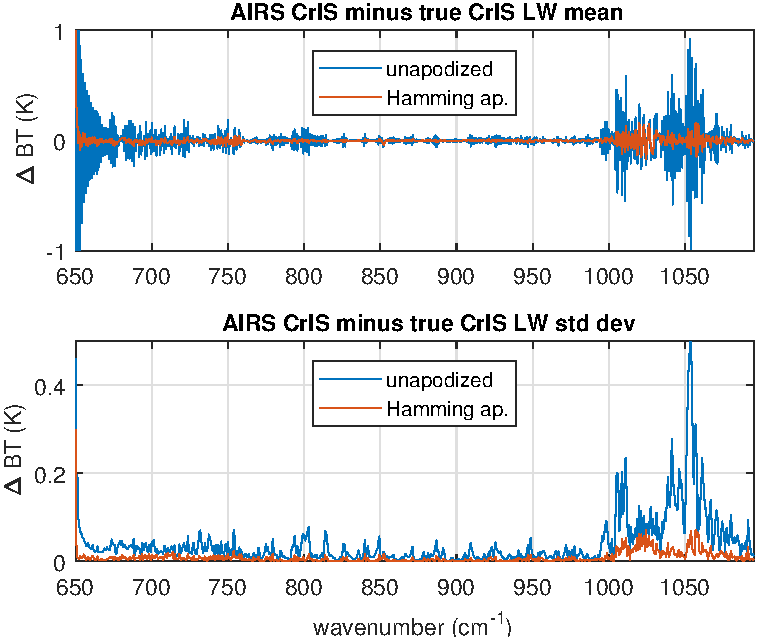
\includegraphics[width=\textwidth]{figures/a2cris_diff_LW.pdf}
  \end{centering}\vspace{3mm}
  Mean and standard deviation of unapodized and Hamming apodized
  {\airs} {\cris} minus true {\cris}, for the {\cris} LW band

\end{column}
\begin{column}{0.5\textwidth}  
  \begin{centering}
  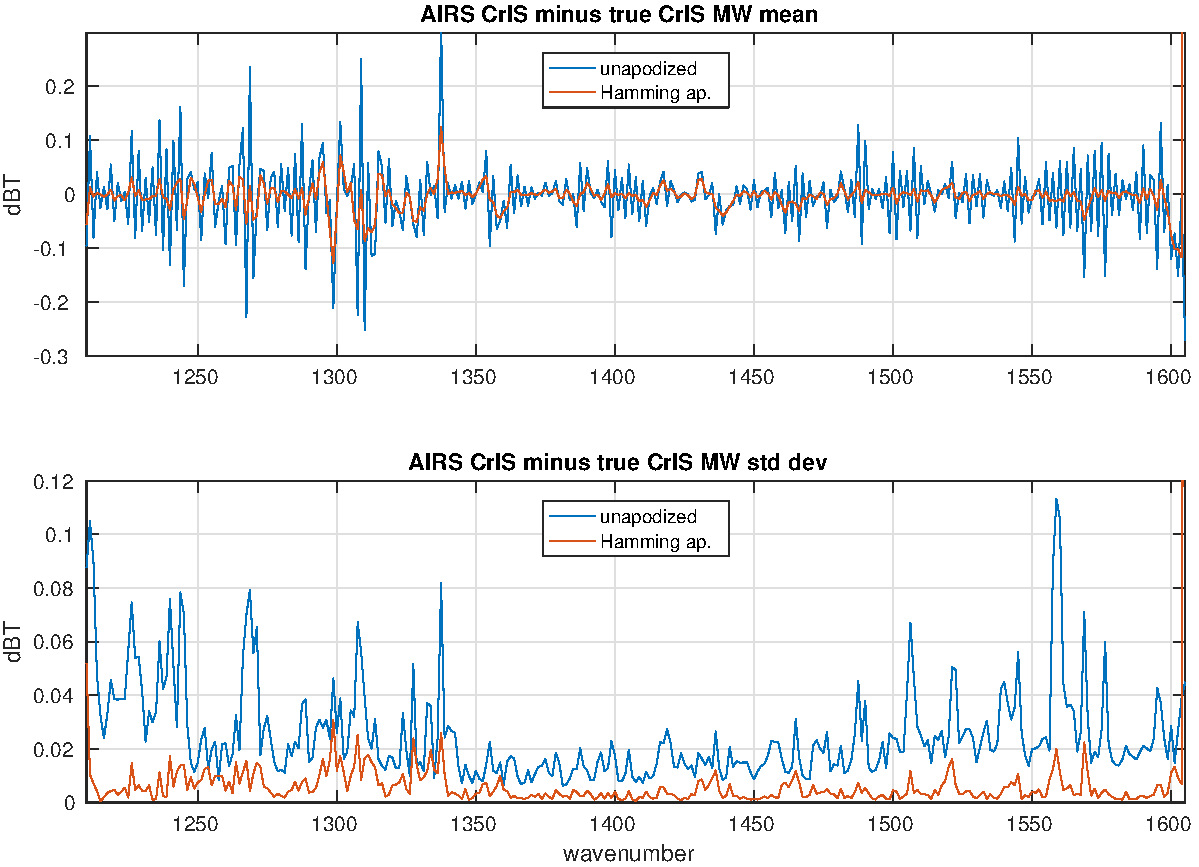
\includegraphics[width=\textwidth]{figures/a2cris_diff_MW.pdf}
  \end{centering}\vspace{3mm}
  Mean and standard deviation of unapodized and Hamming apodized
  {\airs} {\cris} minus true {\cris}, for the {\cris} MW band

\end{column}
\end{columns}
\end{frame}
%----------- slide --------------------------------------------------%
\begin{frame}
\frametitle{AIRS to CrIS residuals}
\begin{columns}[t]
\begin{column}{0.5\textwidth}
  \begin{centering}
  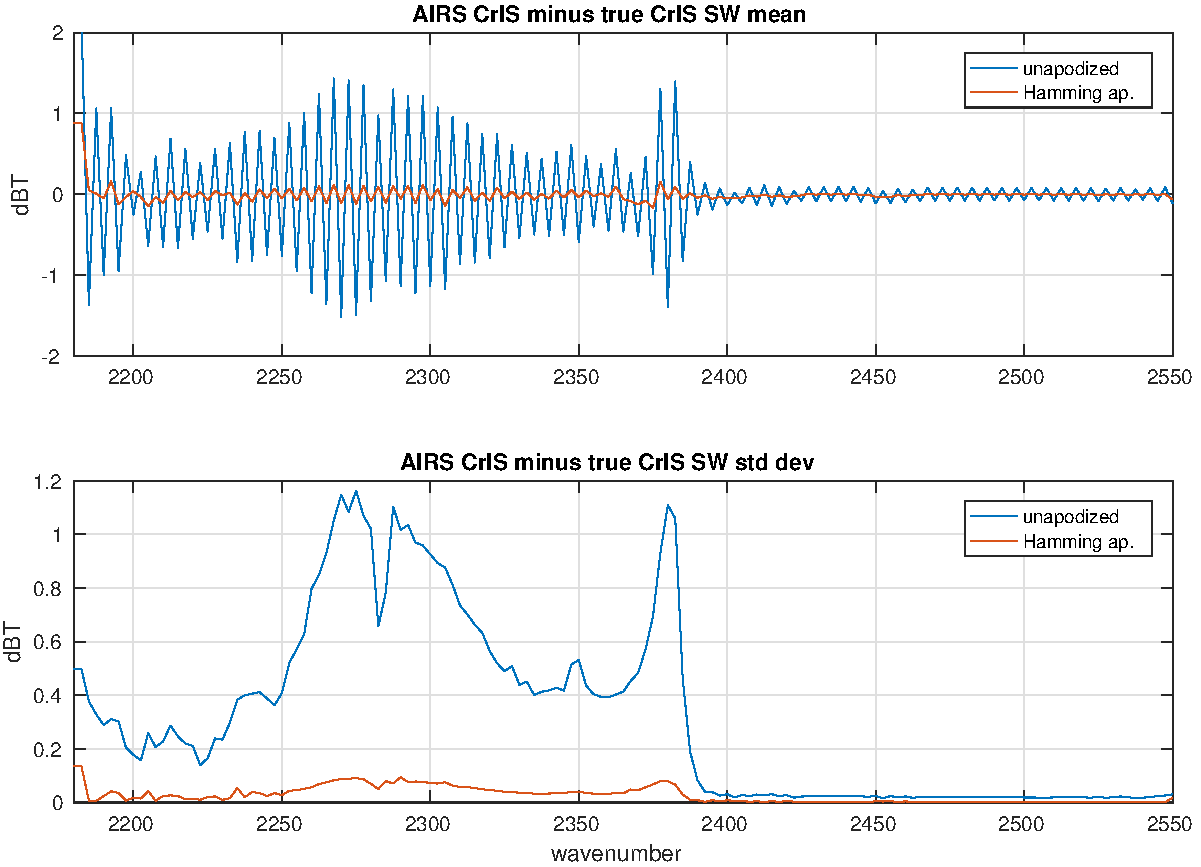
\includegraphics[width=\textwidth]{figures/a2cris_diff_SW.pdf}
  \end{centering}\vspace{3mm}
  Mean and standard deviation of unapodized and Hamming apodized
  {\airs} {\cris} minus true {\cris}, for the {\cris} SW band.

\end{column}
\begin{column}{0.5\textwidth}  
  \begin{centering}
  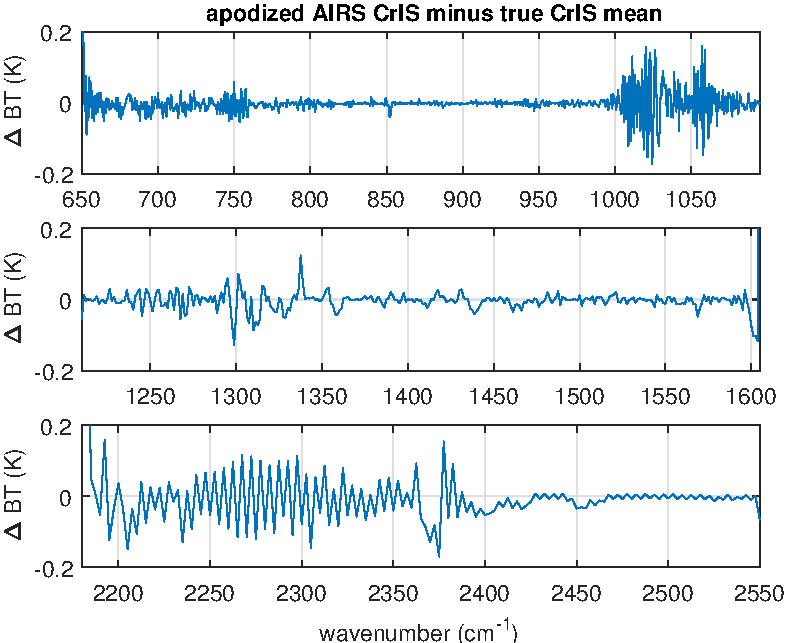
\includegraphics[width=\textwidth]{figures/a2cris_diff_all.pdf}
  \end{centering}\vspace{5mm}
  Mean of apodized residuals for all three {\cris} bands, showing
  the residuals in greater detail.

\end{column}
\end{columns}
\end{frame}
%----------- slide --------------------------------------------------%
\begin{frame}
\frametitle{AIRS to CrIS statistical correction}
\begin{itemize}

  \item We can further reduce the residuals with a simple linear or
    quadratic correction, applied independently to each channel.

  \item We use a set of 7377 radiances calculated from all-sky AIRS
    profiles spanning several consecutive days as the dependent set.

  \item Let $\Ttc_i$ be true {\cris} and $\Tac_i$ {\airs} {\cris}
    brightness temperatures for {\cris} channel $i$, from the
    dependent set.

  \item For the bias test we subtract the mean residual from the
    dependent set.  For the linear test we find $a_i$ and $b_i$ to
    minimize $||a_i\,\Tac_i + b_i - \Ttc_i||_2$, and for the
    quadratic test $c_i$, $a_i$ and $b_i$ to minimize
    $||c_i\,(\Tac_i)^2 + a_i\,\Tac_i + b_i - \Ttc_i||_2$.

  \item The $a$ weights are very close to 1, the $b$ weight to the
    bias, and the $c$ weights to zero.  The linear correction worked
    best.

  \item The resulting correction is applied to the independent set,
    the 49 fitting profiles, for comparison with true {\cris}.  This
    gives a stricter test than splitting the more correlated 7377
    profile set into dependent and independent subsets.

\end{itemize}
\end{frame}
%----------- slide --------------------------------------------------%
\begin{frame}
\frametitle{AIRS to CrIS statistical correction}
\begin{columns}[t]
\begin{column}{0.5\textwidth}
  \begin{centering}
  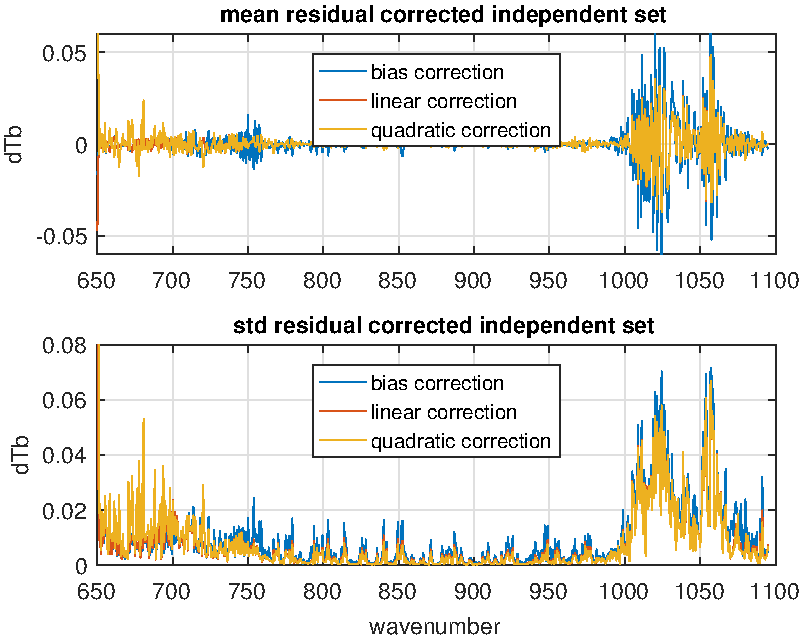
\includegraphics[width=\textwidth]{figures/a2cris_regr_LW.pdf}
  \end{centering}\vspace{3mm}
  Mean and standard deviation of LW corrected apodized residuals.

\end{column}
\begin{column}{0.5\textwidth}
  \begin{centering}
  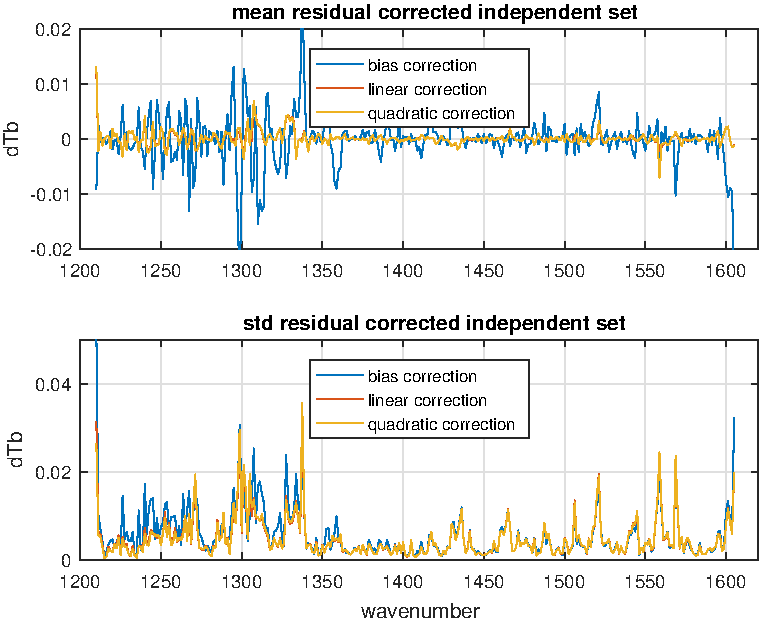
\includegraphics[width=\textwidth]{figures/a2cris_regr_MW.pdf}
  \end{centering}\vspace{3mm}
  Mean and standard deviation of MW corrected apodized residuals.
 
\end{column}
\end{columns}
\end{frame}
%----------- slide --------------------------------------------------%
\begin{frame}
\frametitle{AIRS to CrIS statistical correction}
\begin{columns}[t]
\begin{column}{0.5\textwidth}  
  \begin{centering}
  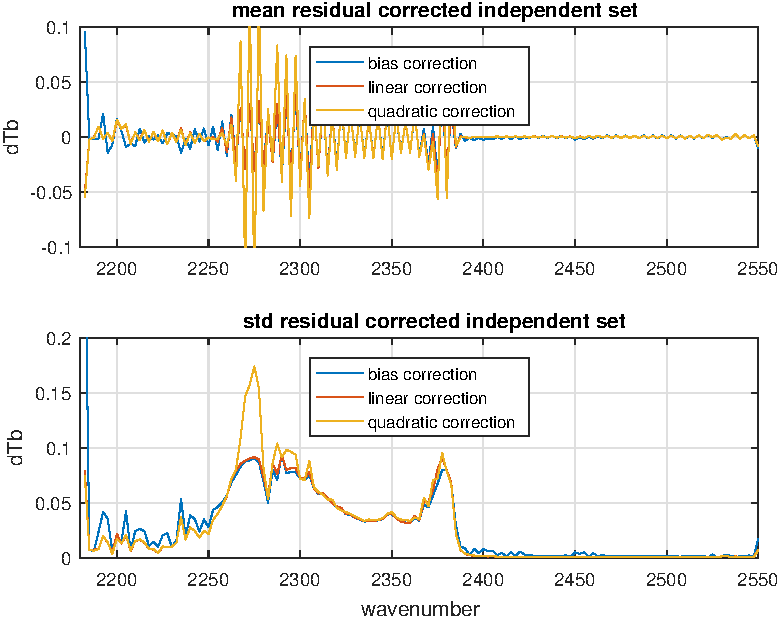
\includegraphics[width=\textwidth]{figures/a2cris_regr_SW.pdf}
  \end{centering}\vspace{3mm}
  Mean and standard deviation of SW corrected apodized residuals.

\end{column}
\begin{column}{0.5\textwidth}
  \begin{centering}
  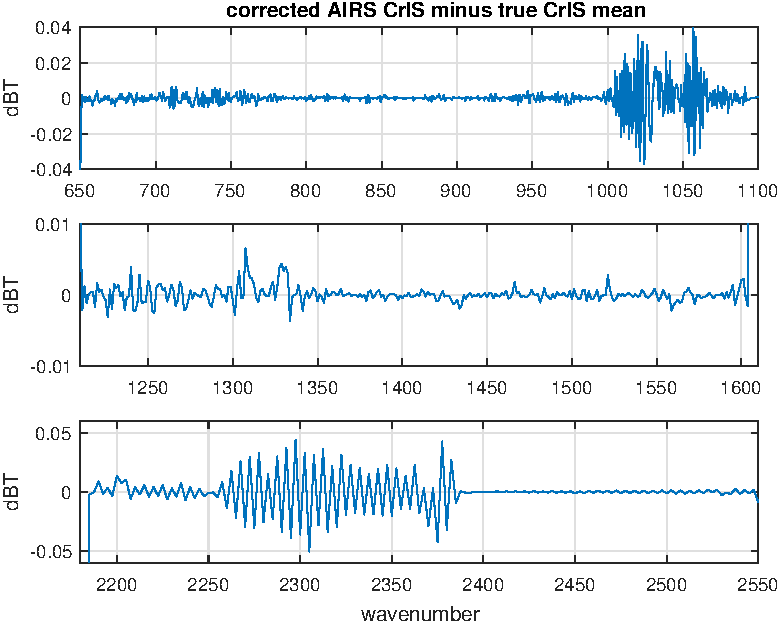
\includegraphics[width=\textwidth]{figures/ap_decon_corr.pdf}
  \end{centering}\vspace{3mm}
  Mean corrected apodized residuals for all three bands, showing
  the linear corrected apodized residuals in greater detail.
\end{column}
\end{columns}
\end{frame}
%----------- slide --------------------------------------------------%
\begin{frame}
\frametitle{NEdN of the translation}
\begin{columns}[t]
\begin{column}{0.5\textwidth}  
  \begin{centering}
  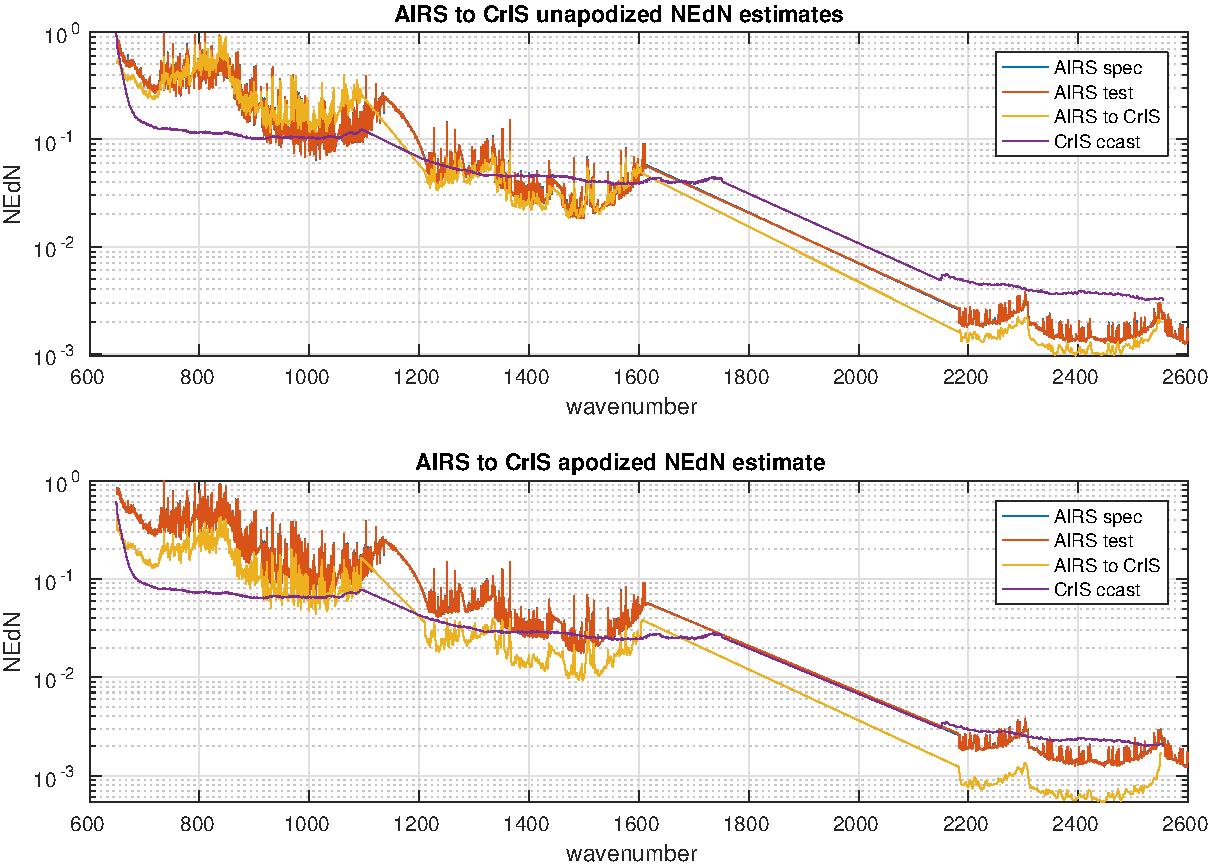
\includegraphics[width=\textwidth]{figures/a2cris_nedn.pdf}
  \end{centering}\vspace{4mm}
  {\airs}, {\airs}-to-{\cris}, and {\cris} NEdN.  Apodization
  reduces the {\cris} and {\airs}-to-{\cris} NEdN by a factor of
  $0.63$.

\end{column}
\begin{column}{0.5\textwidth}
  \begin{centering}
  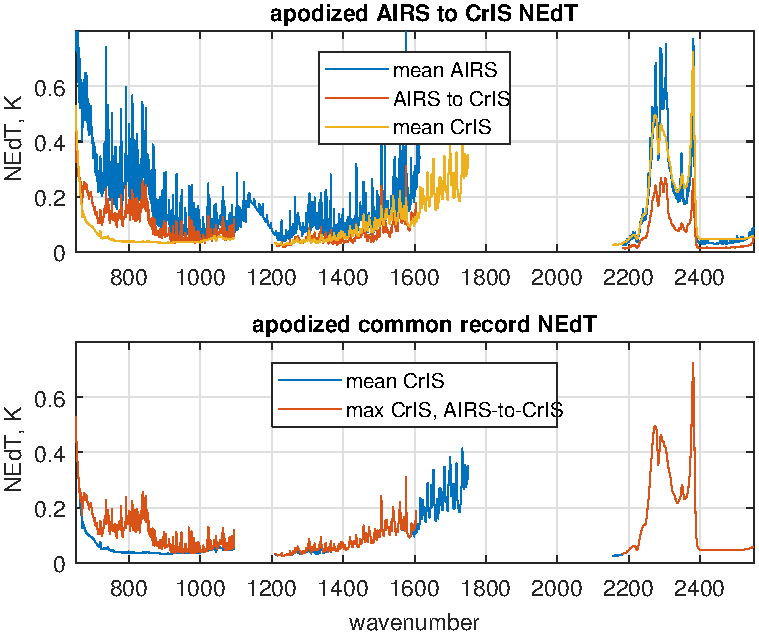
\includegraphics[width=\textwidth]{figures/a2cris_nedt.pdf}
  \end{centering}\vspace{3mm}
  {\airs}, {\airs}-to-{\cris}, and {\cris} apodized NEdT, and the
  max of {\cris} and {\airs}-to-{\cris} NEdT with {\cris} shown as
  a reference.
 
\end{column}
\end{columns}
\end{frame}
%----------- slide --------------------------------------------------%
\begin{frame}
\frametitle{L1c to L1d translation}
\begin{itemize}

  \item The {\airs} deconvolution can be used for other
    translations.

  \item We consider reconvolution to an idealized grating model for
    resolving powers of 700 and 1200.

  \item Define an {\airs} L1d basis with resolving power $R$ using
    the generalized Gaussian described earlier as follows:

  \item Let $v_0$ be the frequency of the first channel, and for
    $i\ge0$ $\fwhm_i = v_i / R$, $dv_i = \fwhm_i / 2$, and $v_{i+1}
    = v_i + dv_i$.

  \item As with tests of the {\airs} to {\cris} translation, we get
    ``true L1d'' by convolving kcarta radiances with an L1d basis at
    the desired resolving power.

  \item {\airs} L1c is translated to L1d by deconvolution to the
    intermediate grid followed by reconvolution to the desired L1d
    basis, and this is compared with true L1d.

  \item A statistical correction similar to that used for the
    {\airs} to {\cris} translation is then applied

\end{itemize}
\end{frame}
%----------- slide --------------------------------------------------%
\begin{frame}
\frametitle{L1c to L1d translation}
\begin{columns}[t]
\begin{column}{0.5\textwidth}
  \begin{centering}
  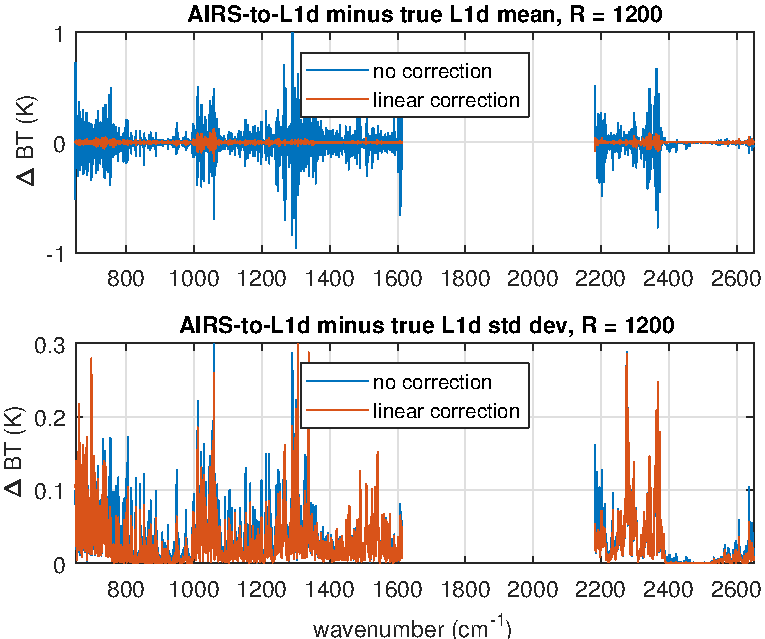
\includegraphics[width=\textwidth]{figures/L1d_cor1_1200.pdf}
  \end{centering}\vspace{3mm}
  Mean and standard deviation over the 49 fitting profiles for the
  L1c to L1d translation minus true L1d, for a resolving power of
  1200.

\end{column}
\begin{column}{0.5\textwidth}  
  \begin{centering}
  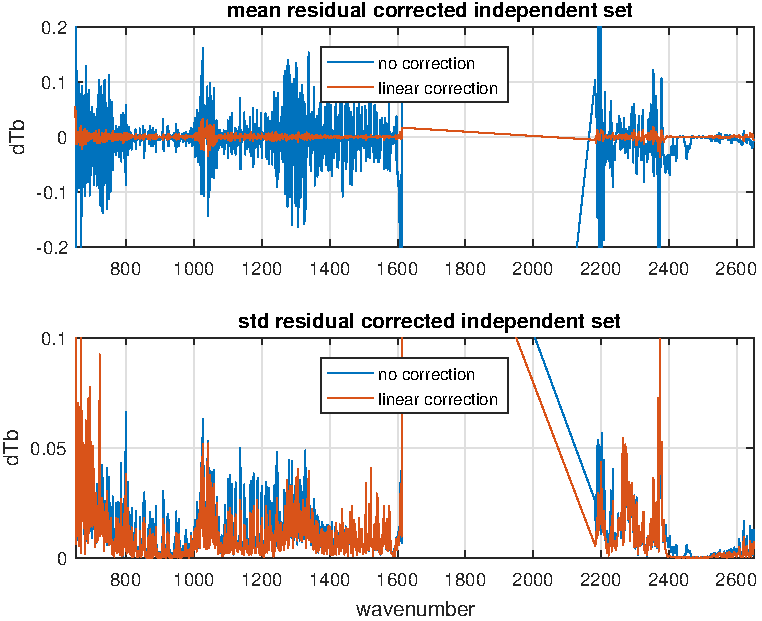
\includegraphics[width=\textwidth]{figures/L1d_cor1_700.pdf}
  \end{centering}\vspace{3mm}
  Mean and standard deviation over the 49 fitting profiles for the
  L1c to L1d translation minus true L1d, for a resolving power of
  700.
 
\end{column}
\end{columns}
\end{frame}
%----------- slide --------------------------------------------------%
\begin{frame}
\frametitle{direct regression}
\begin{itemize}

  \item The {\airs} to {\cris} and {\airs} to L1d translations can
    be represented as a single linear transform, the composition of
    the deconvolution and reconvolution matrices.  

  \item We can get such a one-step tranform in other ways.

  \item For example if $r_a$ and $r_c$ are $m \times k$ and $n
    \times k$ {\airs} and {\cris} radiance sets, we can find an $n
    \times m$ array $X$ to minimize $\|X r_a - r_c\|_2$.

  \item Typically $k > m$, giving an overdetermined system, and we
    solve $r_a^t X^t = r_c^t$ for $X$ by regression.

  \item This differs from the regression corrections used earlier;
    there regression was used to find linear or quadratic correction
    coefficients independently for each channel.

  \item As before we use the 7377 profile set as the dependent and
    the 49 profile as the independent sets.

  \item This approach is prone to over-fitting, and the regression
    matrices show significant off-diagonal correlations.

\end{itemize}
\end{frame}
%----------- slide --------------------------------------------------%
\begin{frame}
\frametitle{direct regression}
\begin{columns}[t]
\begin{column}{0.5\textwidth}
  \begin{centering}
  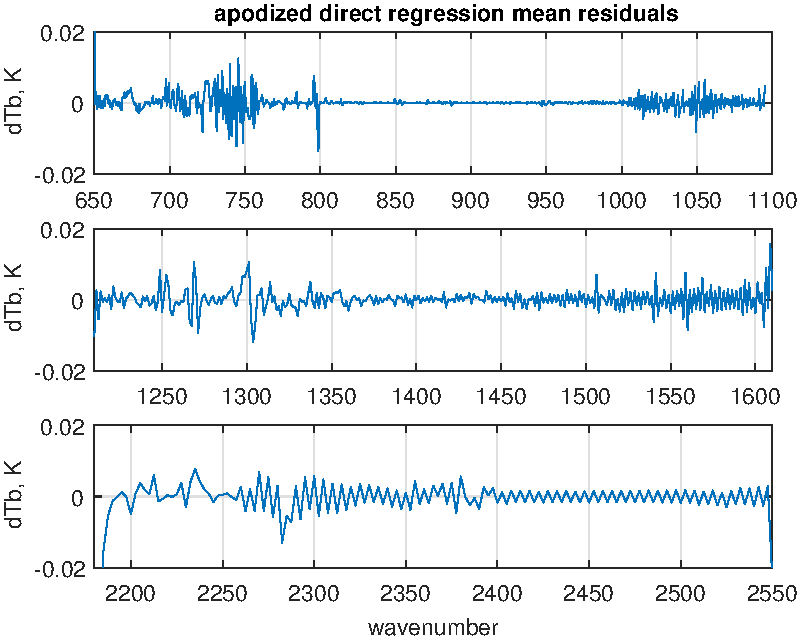
\includegraphics[width=\textwidth]{figures/ap_dir_regr.pdf}
  \end{centering}\vspace{3mm}
  Mean residuals over the 49 profile independent set for {\airs} to
  apodized {\cris} direct regression.

\end{column}
\begin{column}{0.5\textwidth}  
  \begin{centering}
  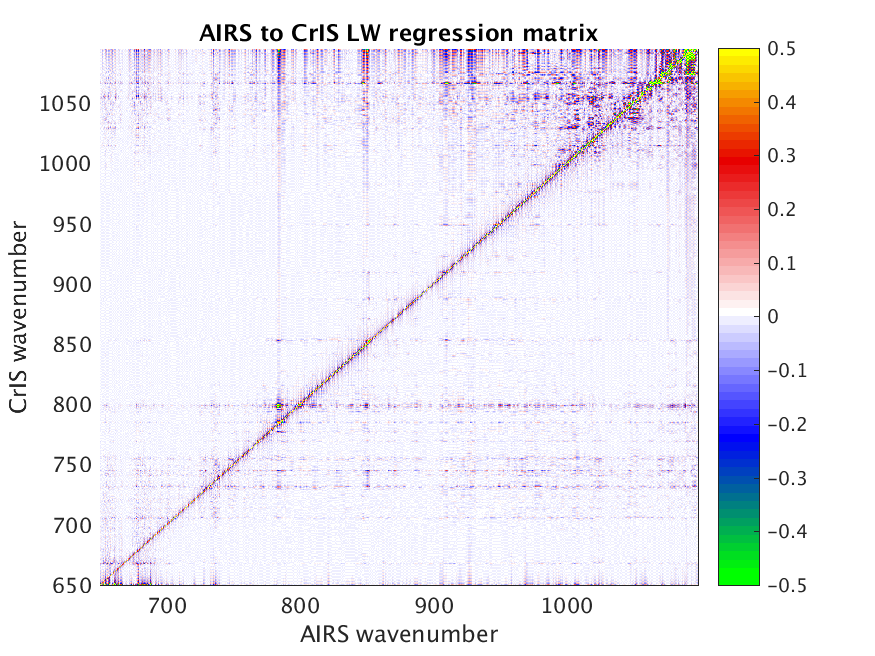
\includegraphics[width=\textwidth]{figures/LW_dir_regr_mat.png}
  \end{centering}\vspace{3mm}
  Regression coefficients from the 7377 profile dependent set for
  the LW direct regression.

\end{column}
\end{columns}
\end{frame}
%----------- slide --------------------------------------------------%
\begin{frame}
\frametitle{principal component regression}
\begin{itemize}

  \item We can use a form of principal component regression to
    reduce unwanted correlations.

  \item Let $r_a$ and $r_c$ be $m \times k$ and $n \times k$ {\airs}
    and {\cris} radiance sets.

  \item Let $r_a = U_a S_a\,V_a^T$ be a singular value decomposition
    with singular values in descending order and $U_a^i$ the first
    $i$ columns of $U_a$.

  \item Similarly let $r_c = U_c S_c\,V_c^T$ be a singular value
    decomposition with singular values in descending order and
    $U_c^j$ the first $j$ columns of $U_c$.

  \item Let $\hat r_a = (U_a^i)^T r_a$ and $\hat r_c = (U_c^j)^T
    r_c$ be $r_a$ and $r_c$ represented with respect to the bases
    $U_a^i$ and $U_c^j$.

  \item Then find $X$ to minimize $\|X \hat r_a - \hat r_c\|_2$ by
    solving $\hat r_a^T X^T = \hat r_c^T$ for $X$ by regression.

  \item This gives us $R = U_c^j X (U_a^i)^T$, an {\airs} to {\cris}
    transform parameterized by the {\airs} and {\cris} basis sizes
    $i$ and $j$.

\end{itemize}
\end{frame}
%----------- slide --------------------------------------------------%
\begin{frame}
\frametitle{principal component regression}
\begin{columns}[t]
\begin{column}{0.5\textwidth}
  \begin{centering}
  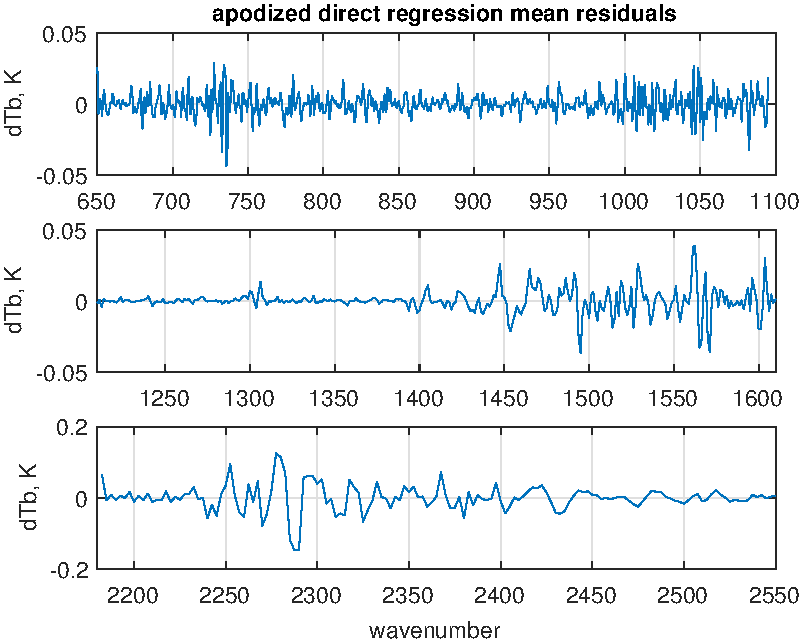
\includegraphics[width=\textwidth]{figures/ap_pc_regr.pdf}
  \end{centering}\vspace{3mm}
  Mean residuals over the 49 profile independent set for {\airs} to
  apodized {\cris} principal component regression.

\end{column}
\begin{column}{0.5\textwidth}  
  \begin{centering}
  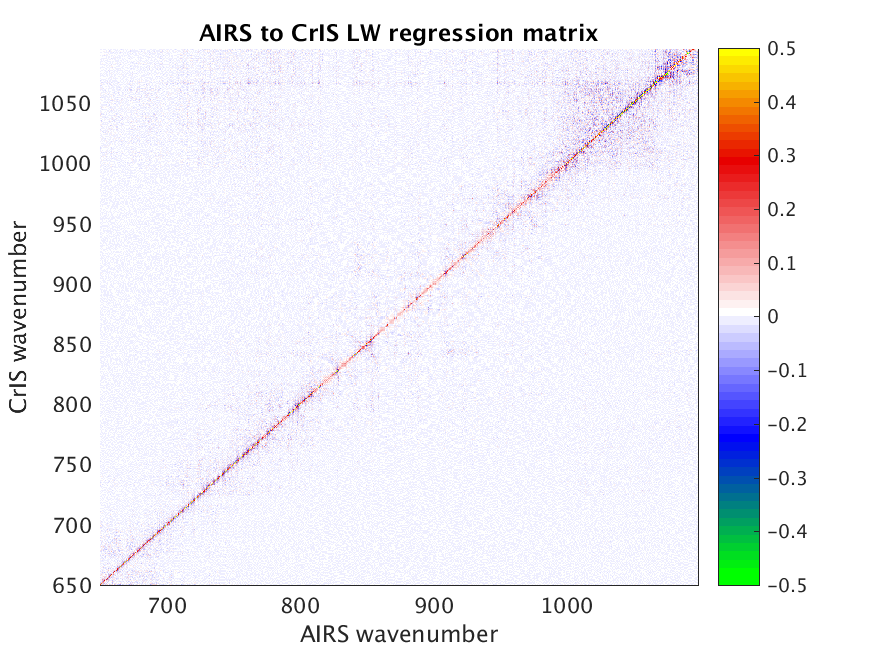
\includegraphics[width=\textwidth]{figures/LW_pc_regr_mat.png}
  \end{centering}\vspace{3mm}
  Regression coefficients from the 7377 profile dependent set for
  LW principal component regression with $i = j = 500$.
 
\end{column}
\end{columns}
\end{frame}
%----------- slide --------------------------------------------------%
\begin{frame}
\frametitle{principal component regression}
\begin{columns}[t]
\begin{column}{0.5\textwidth}
  \begin{centering}
  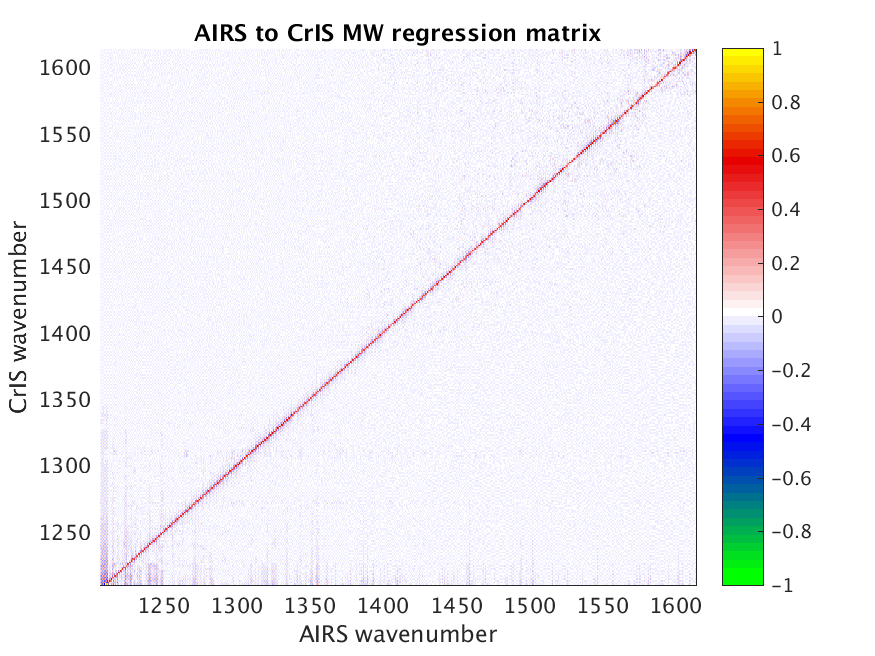
\includegraphics[width=\textwidth]{figures/MW_pc_regr_mat.png}
  \end{centering}\vspace{3mm}
  Regression coefficients from the 7377 profile dependent set for
  MW principal component regression with $i = 500$ and $j = 320$.
 
\end{column}
\begin{column}{0.5\textwidth}  
  \begin{centering}
  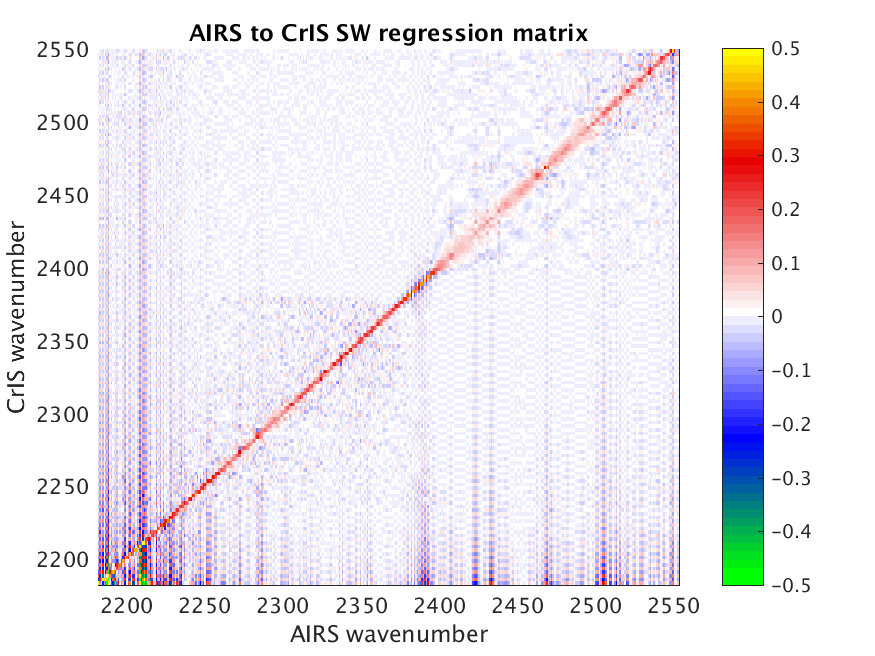
\includegraphics[width=\textwidth]{figures/SW_pc_regr_mat.png}
  \end{centering}\vspace{3mm}
  Regression coefficients from the 7377 profile dependent set for
  SW principal component regression with $i = j = 100$.

\end{column}
\end{columns}
\end{frame}
%----------- slide --------------------------------------------------%
\begin{frame}
\frametitle{conclusions}
\begin{itemize}

  \item The {\airs} deconvolution gives a modest resolution
    enhancement, at the cost of added artifacts and noise.

  \item The deconvolution can be used for other translations, such
    as an idealized grating model.

  \item {\airs} to {\cris} translation via deconvolution,
    reconvolution, and a statistical correction works better than
    translation via regular or principal component regression.

  \item Translation via deconvolution works significantly better
    than conventional interpolation, including interpolation to the
    intermediate grid followed by convolution to the final target.

  \item This talk, a more in-depth companion paper, and all the
    translation and test code discussed here are available online at
    github:
    \begin{itemize}
      \item https://github.com/motteler/decon\_paper
      \item https://github.com/strow/airs\_deconv
      \item https://github.com/strow/iasi\_decon
    \end{itemize}

\end{itemize}
\end{frame}
%----------- slide --------------------------------------------------%

\end{document}

